
\documentclass{beamer}

\mode<presentation>{\usetheme{Madrid}}

\usepackage[utf8]{inputenc}
\usepackage[ngerman]{babel}
\usepackage{amsmath, amssymb, amsthm}
\usepackage{graphicx}
\usepackage{booktabs}
\usepackage{tikz}
\usetikzlibrary {automata}
\usepackage{stmaryrd}
\usepackage{subfig}


\author[Philipp Geier]{}
\title[Sorting Colored Balls in Colored Tubes]{Sorting Colored Balls in Colored Tubes \\ von Ernst Althaus et. al}
\institute[Universität Trier]{}
\date{}
\beamertemplatenavigationsymbolsempty

\usepackage{enumitem}
\newlist{arrowlist}{itemize}{1}
\setlist[arrowlist]{label=$\Rightarrow$}
\newlist{pointlist}{itemize}{1}
\setlist[pointlist]{label=$\circ$}
\newlist{enumlist}{enumerate}{1}
\setlist[enumlist]{label=\arabic*.}

%—-------------------------------------------------------------

\begin{document}
{
  \usebackgroundtemplate{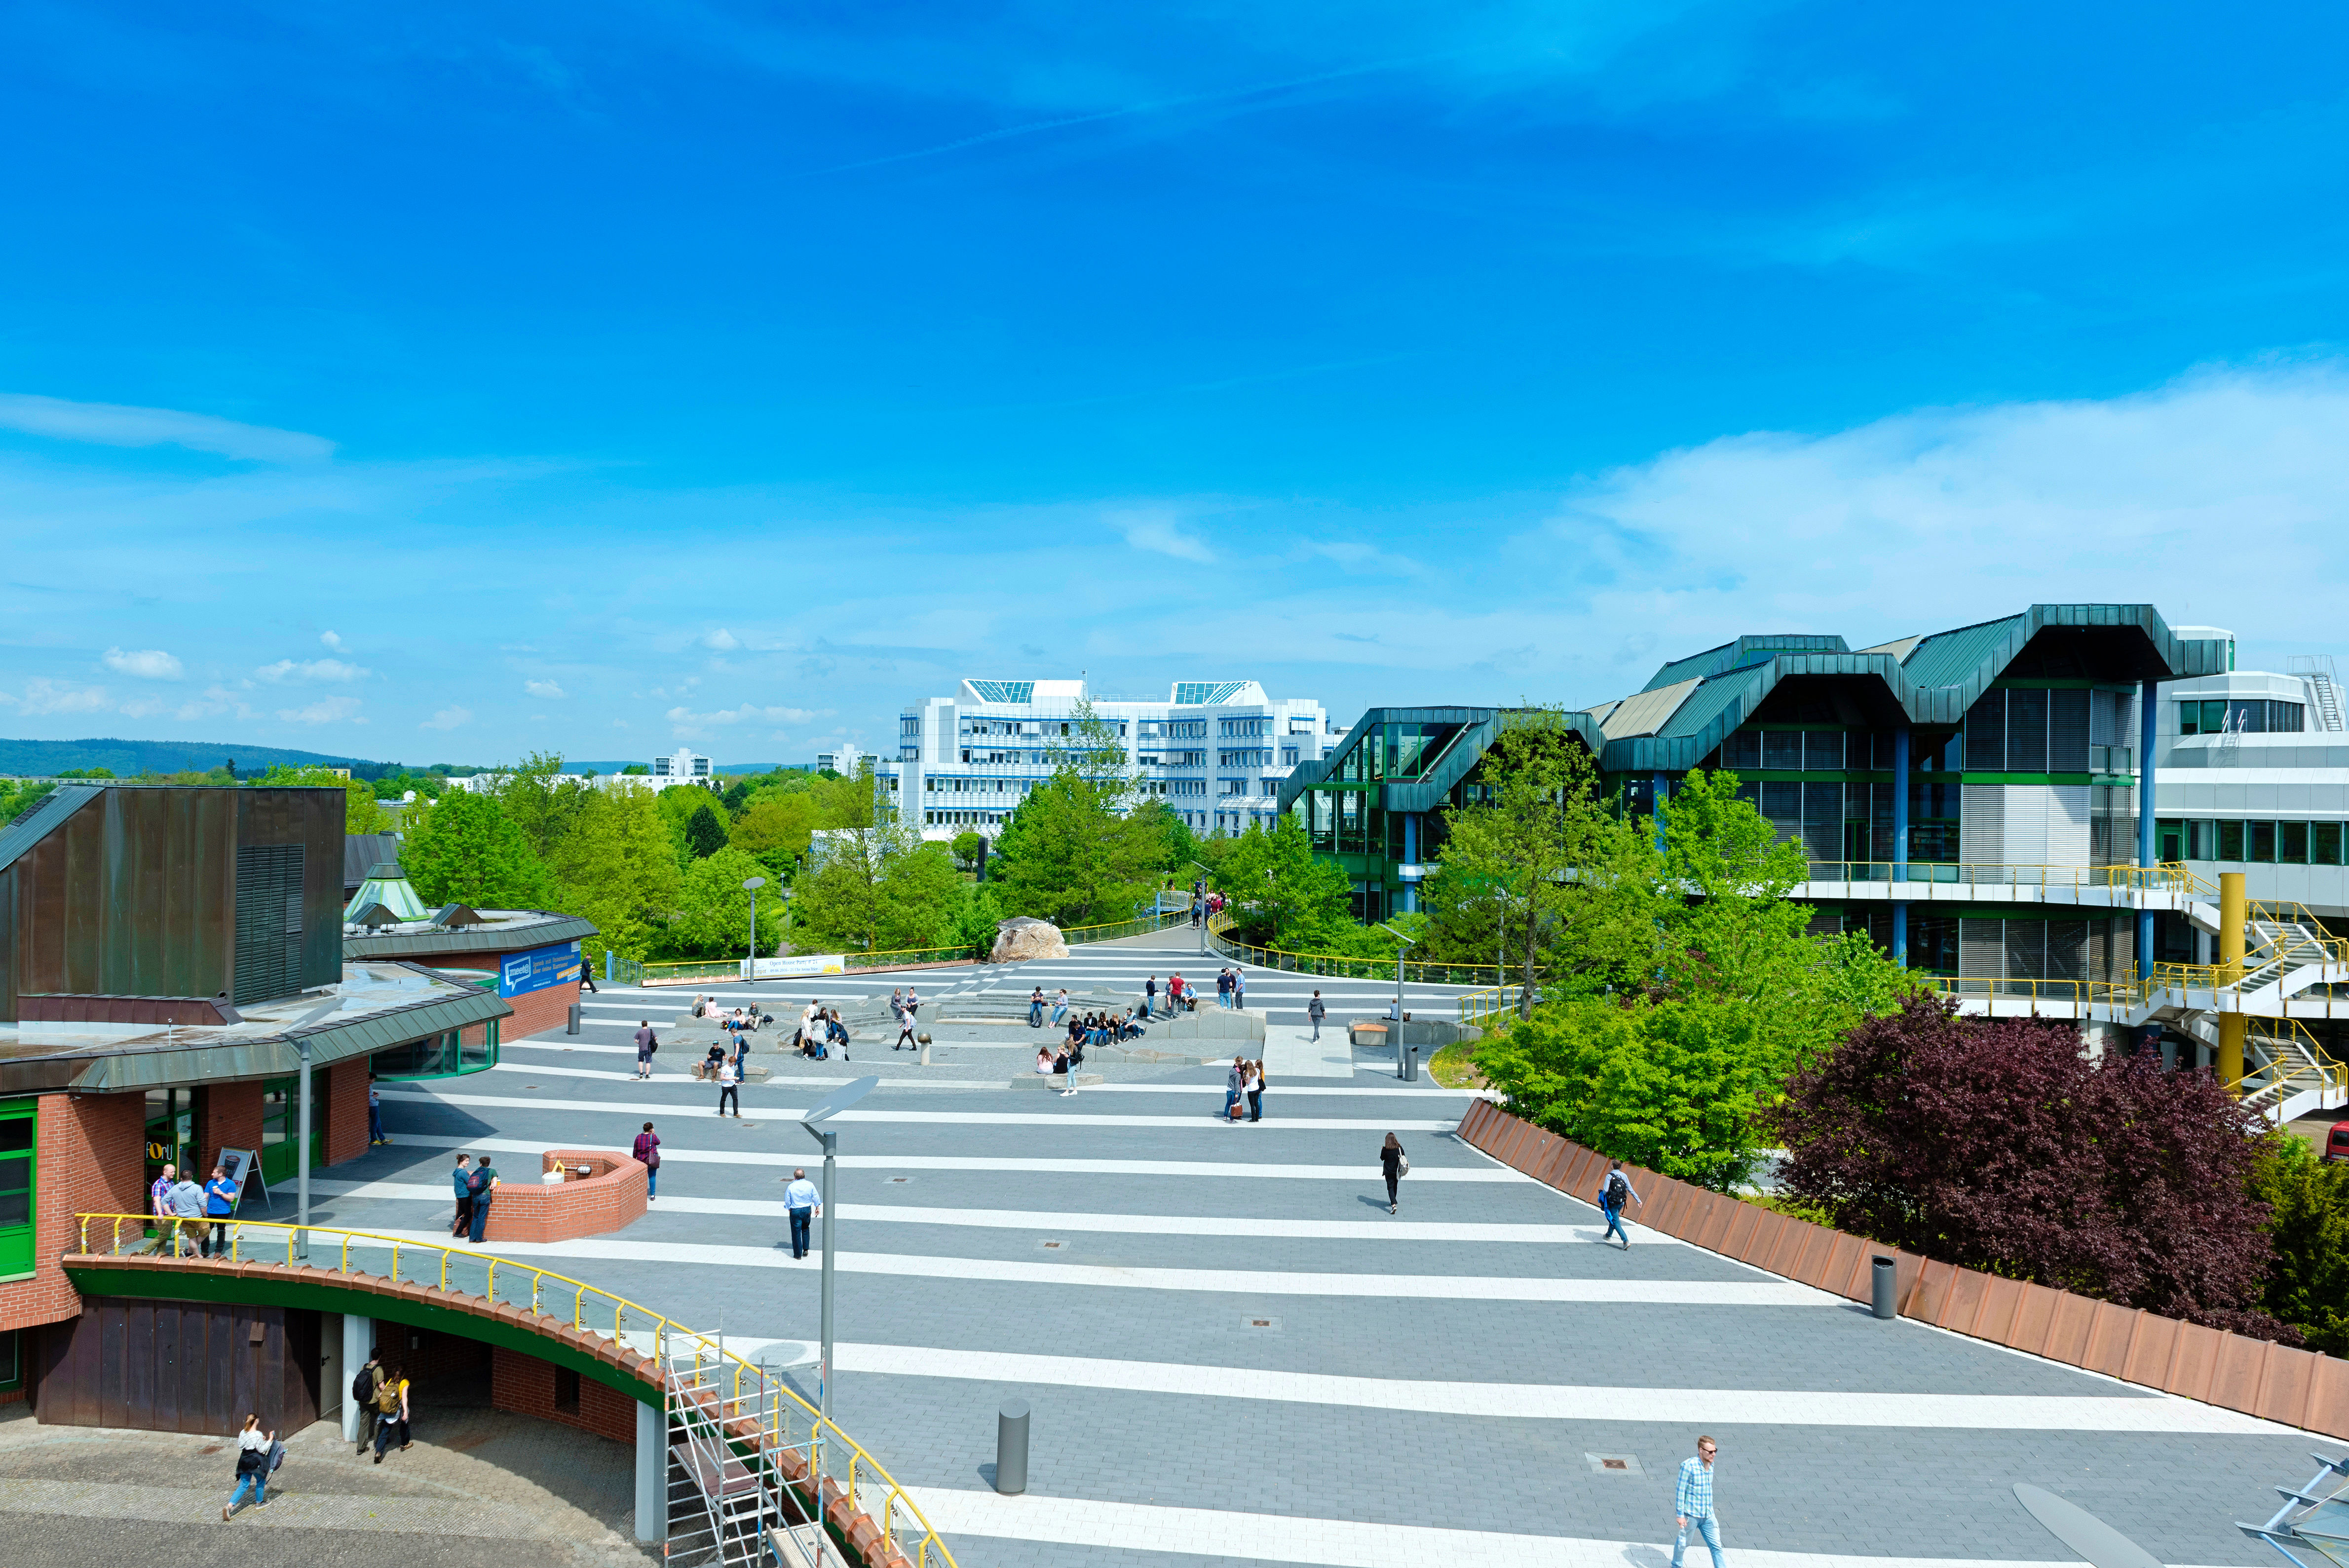
\includegraphics[width=1.2\paperwidth]{unitrier}}
  \begin{frame}
    \maketitle
  \end{frame}
}
    
    %\begin{frame}
       % \frametitle{Inhalt}
		%\tableofcontents
	%\end{frame}
	
%—------------------------------------------------------

\section*{Idee}
\begin{frame}{Idee}
	\begin{figure}[ht]
		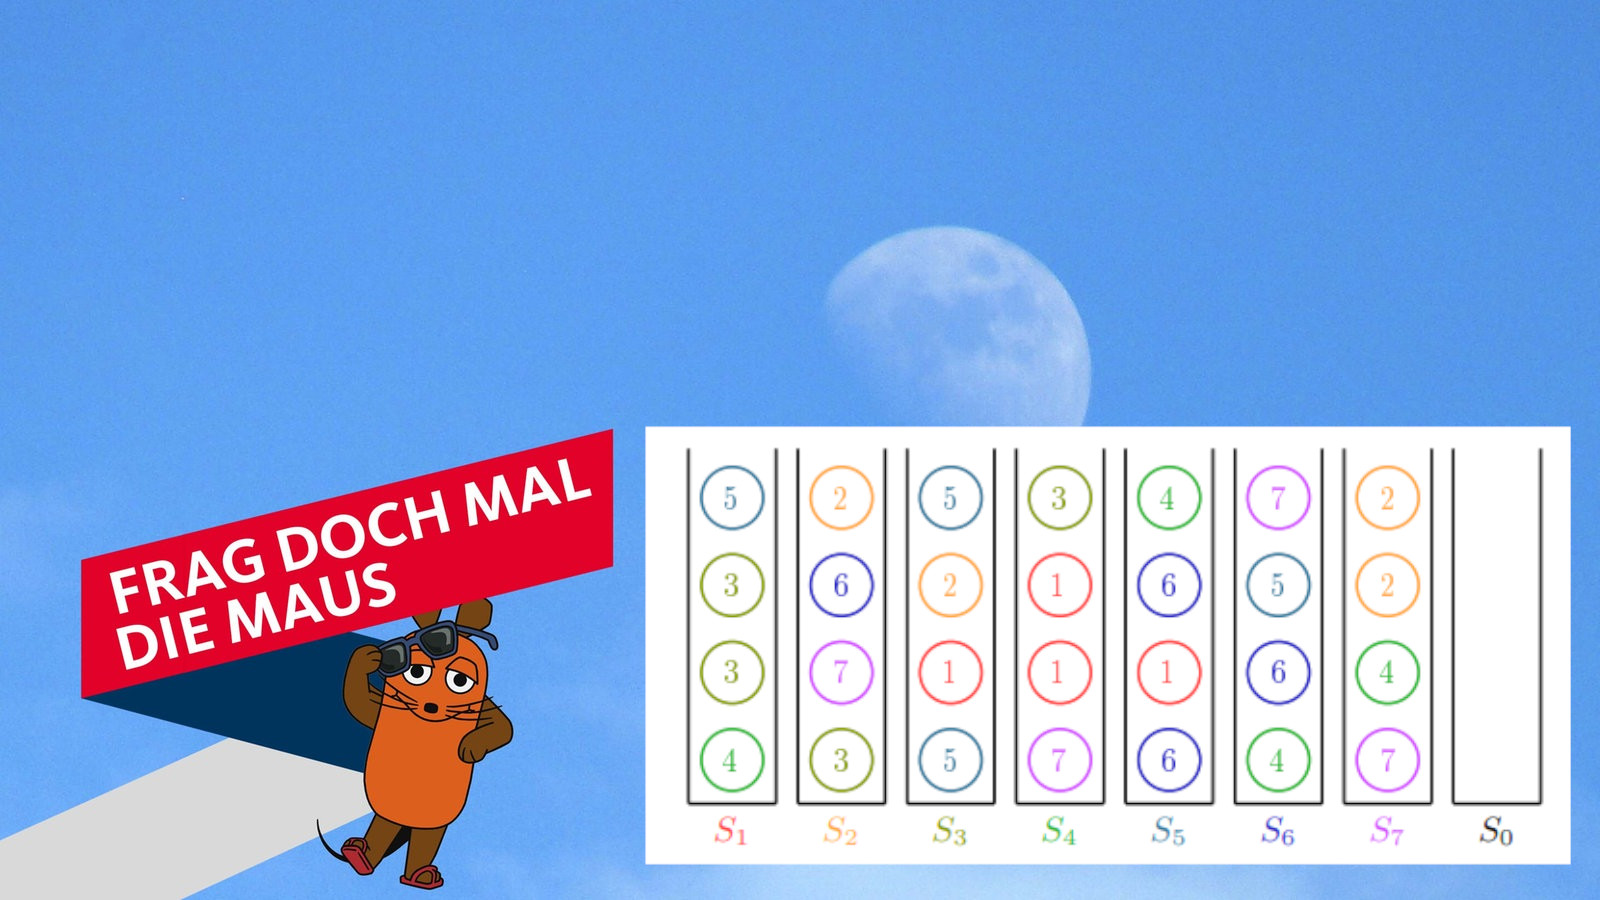
\includegraphics[width=\textwidth]{maus}
    \end{figure}
\end{frame}

\begin{frame}{Idee}
	\begin{pointlist}
		\item Feedback Arc Set Problem (FAS) ist ähnlich zum Spiel mit unbegrenzter Höhe
		\item Konstruktion des Spiels (SCBT) als Graphen 
		\item Reduktion des Problems auf FAS
		\item FAS ist NP-vollständig, somit auch SCBT
	\end{pointlist}
\end{frame}

\section*{Related Work}
\begin{frame}{Related Work}
	\begin{pointlist}
		\item Sortieren von farbigen Bällen in farblosen Tuben. Bälle nur auf Bälle gleicher Farbe oder in leere Tuben (Reduktion von 3-Partition)
	\end{pointlist}
\end{frame}

\begin{frame}{Related Work}
	\begin{pointlist}
		\item $k$ $i$-farbige Bälle in umgekehrter Reihenfolge. Nur adjazente Bälle können getauscht werden 
	\end{pointlist}
	\begin{figure}[ht]
		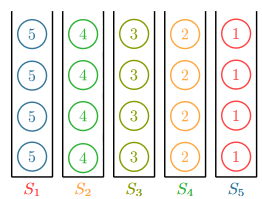
\includegraphics[width=.65\textwidth]{relatedwork}
		\caption{Konstruktion}
    \end{figure}
\end{frame}

\begin{frame}{Related Work}
	\begin{pointlist}
		\item Reales Problem: Container in Terminalen
	\end{pointlist}
	\begin{figure}[ht]
		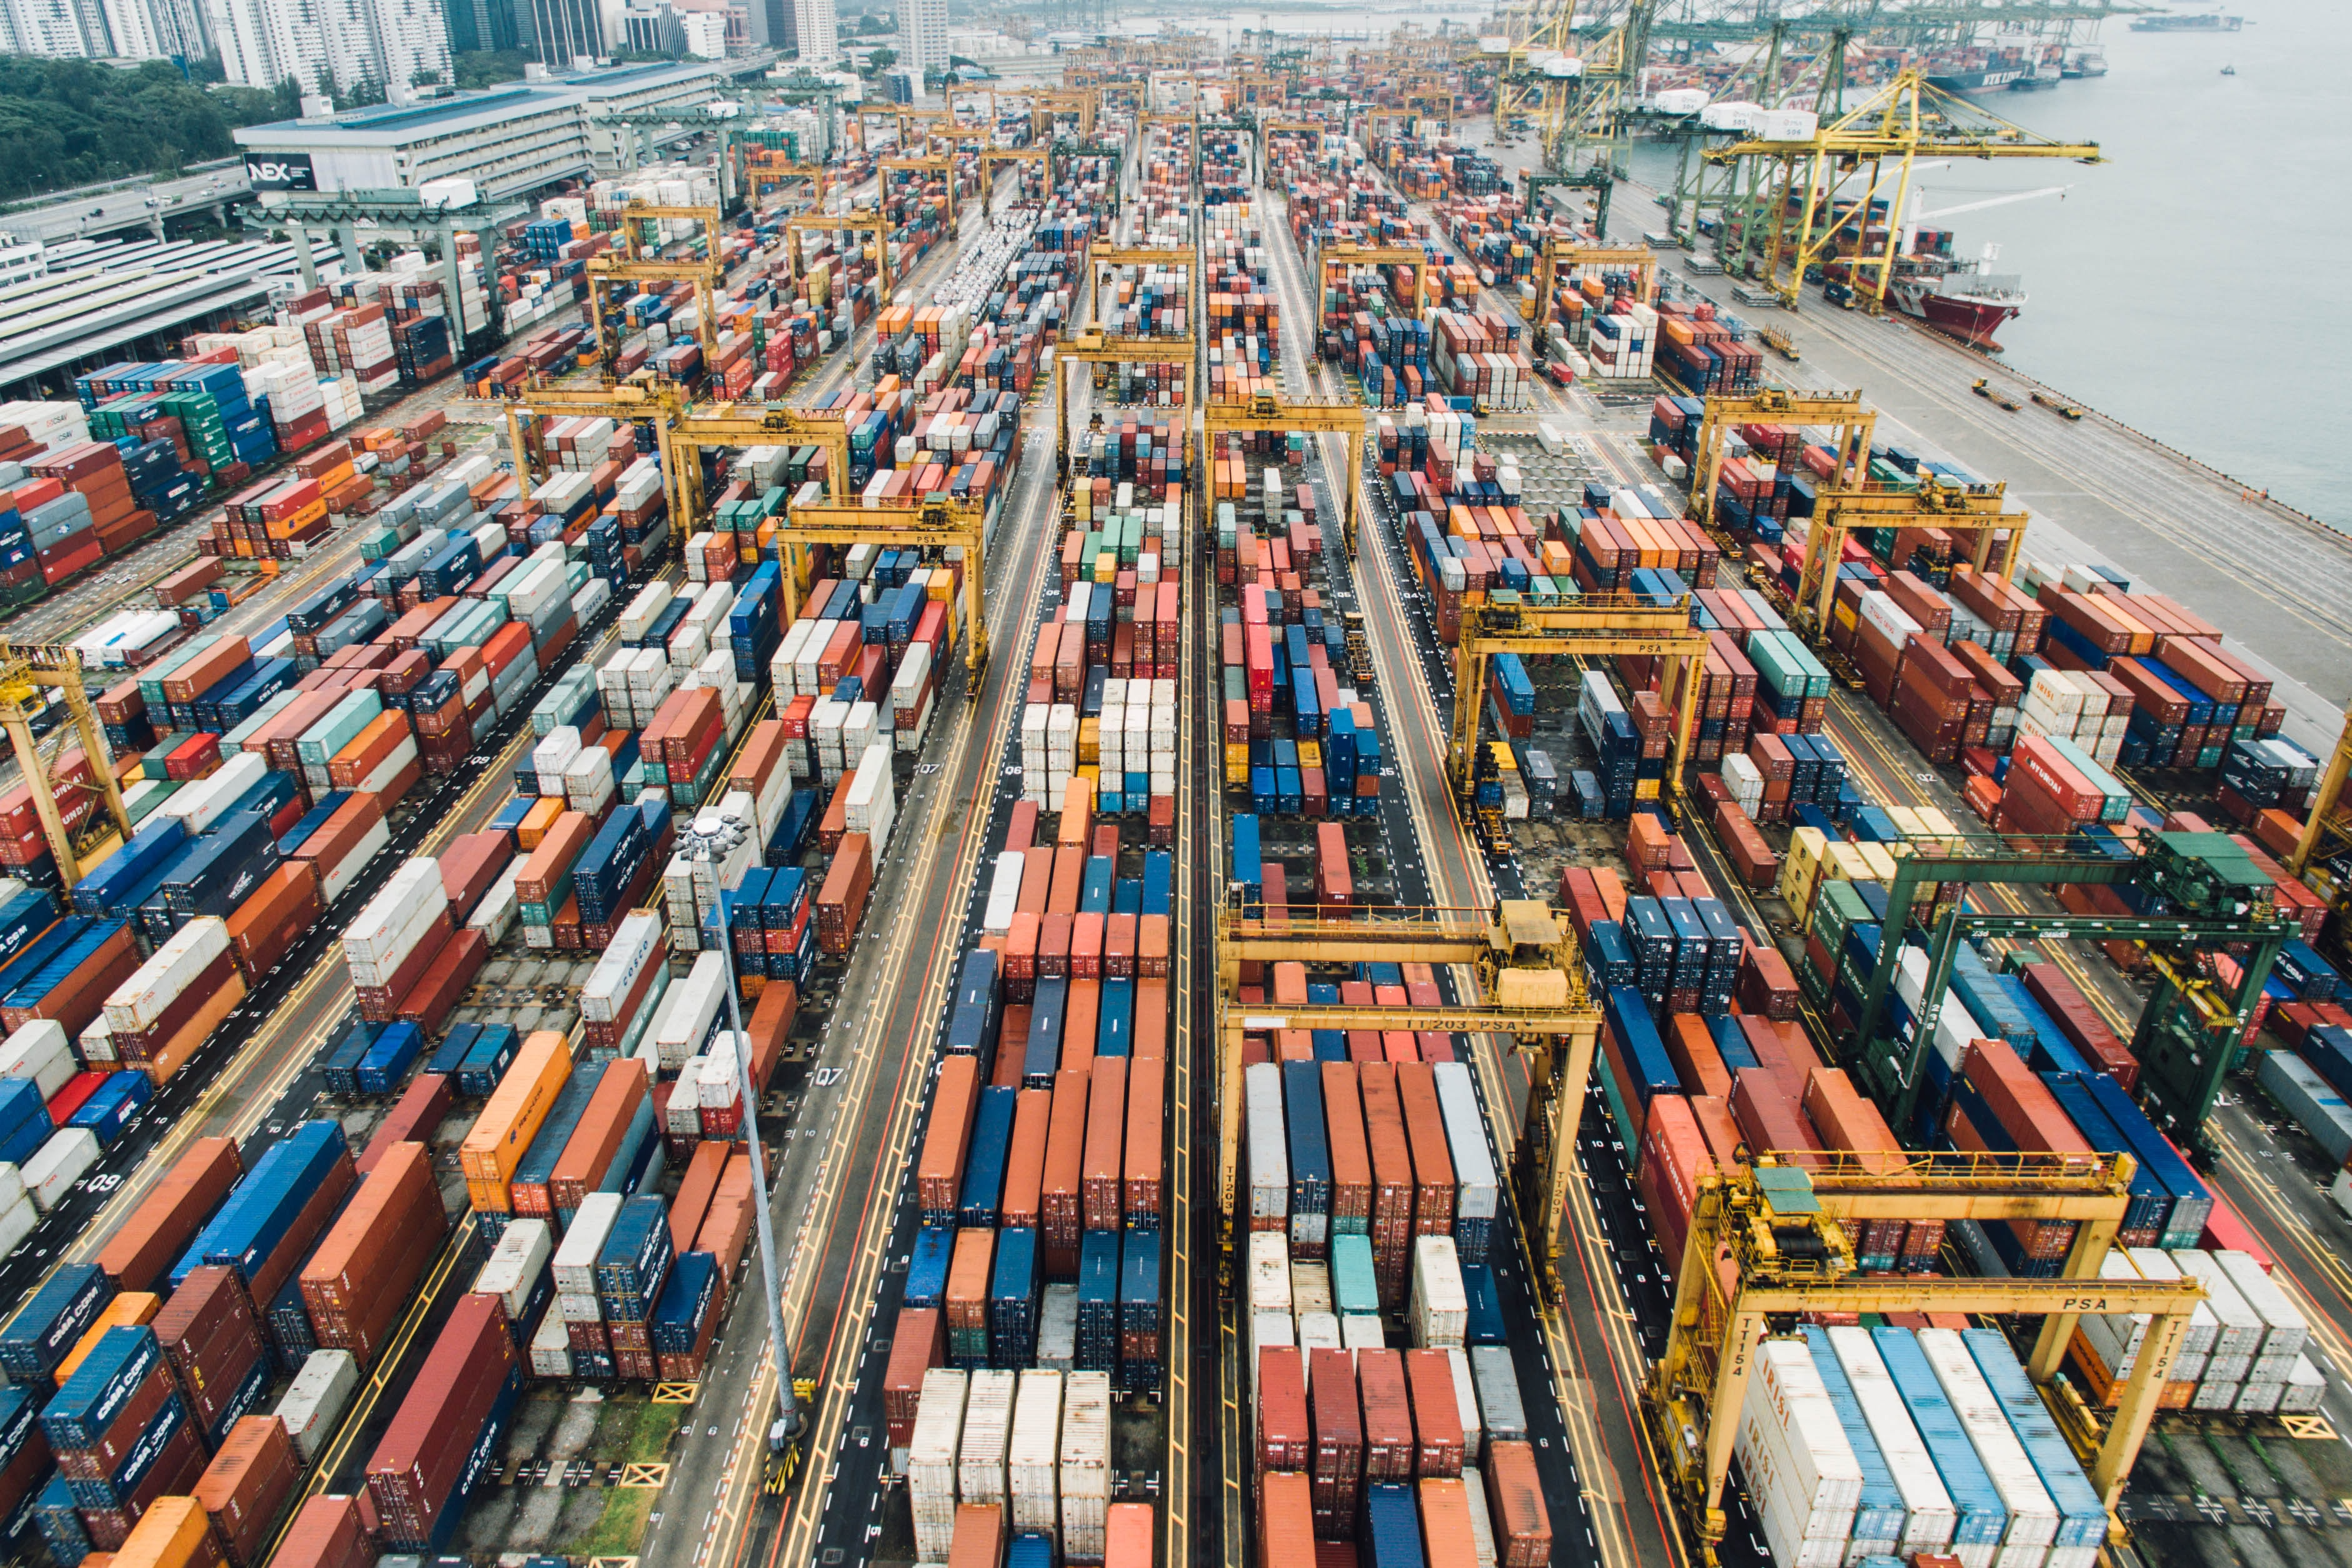
\includegraphics[width=.65\textwidth]{container}
		\caption{Container Terminal}
    \end{figure}
\end{frame}

\section*{Definition}
\begin{frame}{Definitionen}
	\begin{pointlist}
		\item Menge an Farben $C=\{1,\dots c\}$ mit festem $c\in \mathbb{N}$
		\item $c+1$ Tuben der Höhe $h_i\in\mathbb{N}$ in den Farben und eine farblos
		\end{pointlist}
		
\begin{figure}[ht]
		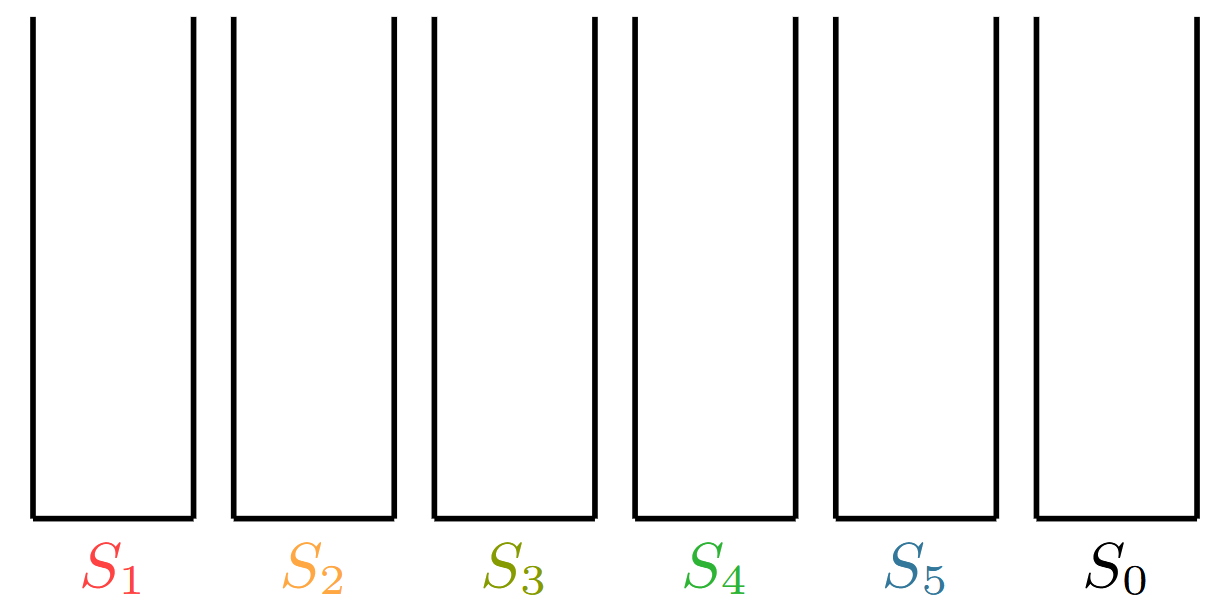
\includegraphics[width=.65\textwidth]{def0}
		\caption{Definition}
    \end{figure}
		\end{frame}
		
		\begin{frame}{Definitionen}
	\begin{pointlist}
		\item Bis zu $h_i$ Bälle pro Farbe $i$
		\item Konfiguration $S_i$ einer Tube ist eine Sequenz $(b_1,\dots,b_l)$ mit $l\leq h_i$
		\item Die farbigen Tuben $T_i$ und die Ersatztube $T_0$ bilden das Tube-Rack $(T_1,\dots,T_c, T_0)$ mit dem Höhenprofil $H=(h_1,\dots,h_c, h_0)$
		\end{pointlist}
		
\begin{figure}[ht]
		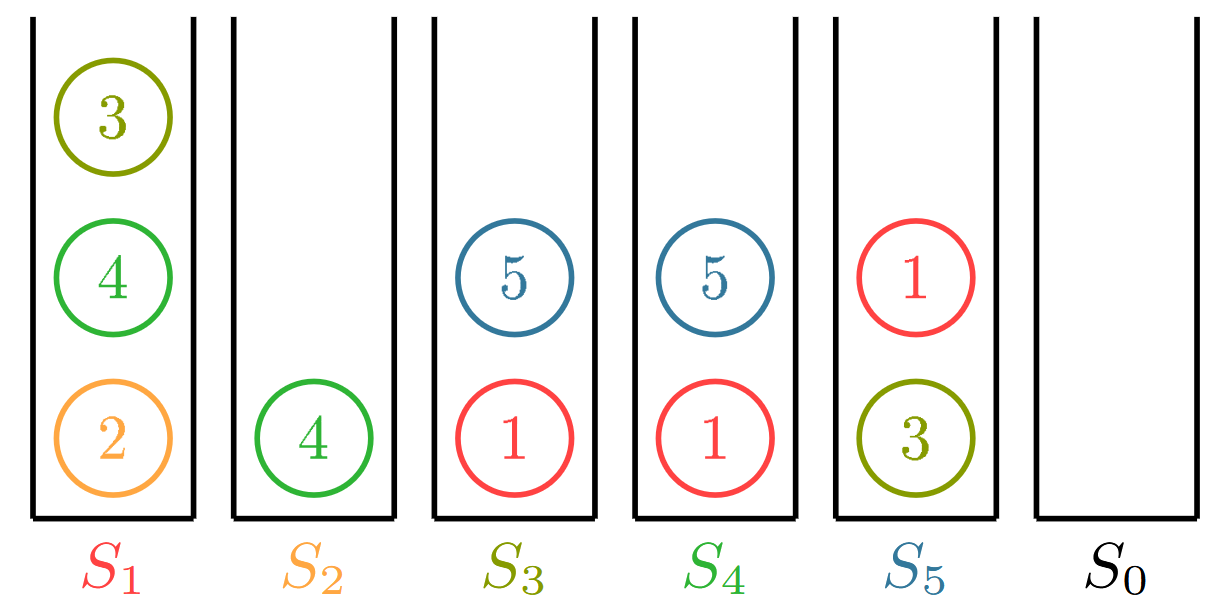
\includegraphics[width=.65\textwidth]{def}
		\caption{Definition}
    \end{figure}
		\end{frame}
		
		
\begin{frame}{Definitionen}
	\begin{pointlist}
		\item Konfiguration eines Tube-Racks ist $S=(S_1,\dots,S_c, S_0)$ mit $|S_i| \leq h_i$
		\item Zug $(i,j)$ heißt valide, falls $|S_i|\geq 1$ und $|S_j| < h_j$
		\item Finale Konfiguration ist $S=(S_i, \dots, S_i, S_0)$ mit $S_0 = ()$ und $S_i =(i,\dots,i)$ für $1\leq i \leq c$
		\item $i$-farbiger Ball ist in finaler Position, falls er in Tube $i$ ist und alle Bälle darunter Farbe $i$ haben
	\end{pointlist}
\end{frame}

\begin{frame}{Probleme}
	\begin{pointlist}
		\item SCBT-Problem:
		\begin{arrowlist}
 			\item Instanz $(H,S,k)$ mit $k$ validen Zügen
		\end{arrowlist}
		\item Restricted SCBT-Problem (RSCBT):
		\begin{arrowlist}
 			\item Instanz $(H,S,k)$ mit $k$ validen Zügen
 			\item Anzahl Bälle der Farbe $i$ gleich der Höhe $h\in\mathbb{N}$ mit dem Höhenprofil $H=(h,\dots,h)$
		\end{arrowlist}
	\end{pointlist}
\end{frame}

\section*{Lemma 1}
\begin{frame}{Lemma 1}
\begin{enumlist}
\item Falls die Anzahl der $i$-farbigen Bälle $h$ entspricht für alle $1 \leq i \leq c$, hat $((h,\dots,h),S,c\cdot h\cdot (2h+1))$ eine Lösung, 
\item Falls $(H,S,k)$ eine Lösung hat und $H' \geq H$ gilt, dann hat $(H',S,k)$ auch eine Lösung
\item Falls $(H,S,k)$ mit $H=(\infty,\dots, \infty)$ eine Lösung hat, dann existiert eine Lösung mit: \begin{pointlist}
\item Bälle in finaler Position werden nicht bewegt
\item Jeder andere wird 1- oder 2-mal bewegt
\end{pointlist}
\item Falls $((\infty, \dots,\infty),S,k)$ eine Lösung hat und $H=( h_1,\dots, h_c, \infty)$ mit $h_i \geq \max(|s_i|,b_i)$ gilt, dann hat $(H,S,k)$ eine Lösung
\end{enumlist}
\end{frame}

\section*{FAS}
\begin{frame}{Feedback Arc Set (FAS)}
\begin{pointlist}
\item geg.: gerichteter Multigraph G=(V,E) und $k\in\mathbb{N}_0$
\item ges.: $\exists E' \subseteq E$ mit $|E'|\leq k$, sodass $G'(V,E\backslash E')$ azyklisch ist
\begin{arrowlist}
\item Nach Karp (1972) NP-vollständig
\end{arrowlist}
\end{pointlist}
\end{frame}

\section*{Konstruktion}
\begin{frame}{Konstruktion}
\begin{pointlist}
\item Wir können aus jedem Graphen ein SCBT Problem machen
\end{pointlist}
\end{frame}

\begin{frame}{Konstruktion}
\begin{pointlist}
\item $V=\{1,\dots,n\}$ mit $c=n$
\item Eine Tube $S_u$ für jeden Knoten $u\in V$
\end{pointlist}
\begin{figure}[ht]
		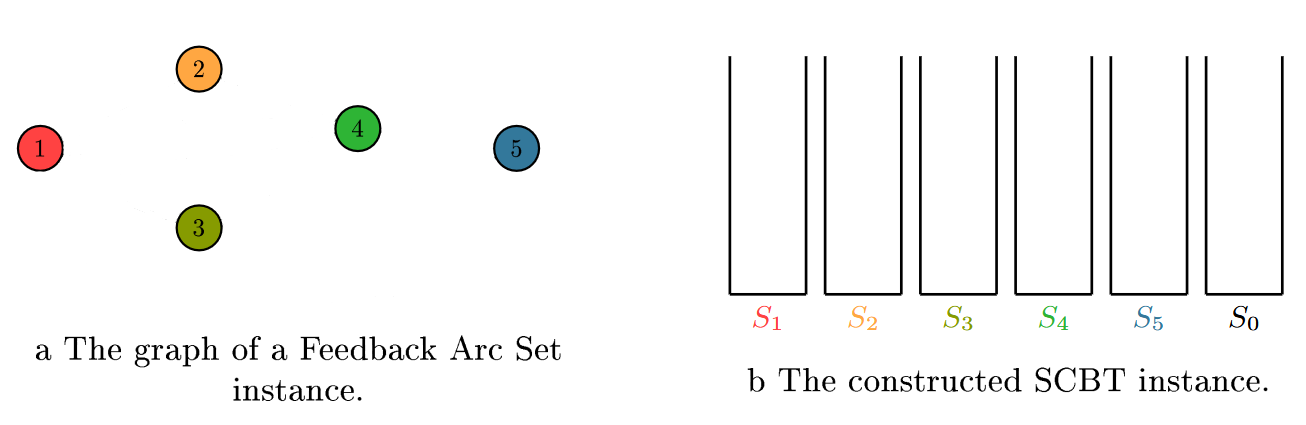
\includegraphics[width=\textwidth]{construct10}
		\caption{Konstruktion}
    \end{figure}
\end{frame}

\begin{frame}{Konstruktion}
\begin{pointlist}
\item Ein Ball der Farbe $u$ in Tube $v$ für jede Kante $(u,v)\in E$
\end{pointlist}
\begin{figure}[ht]
		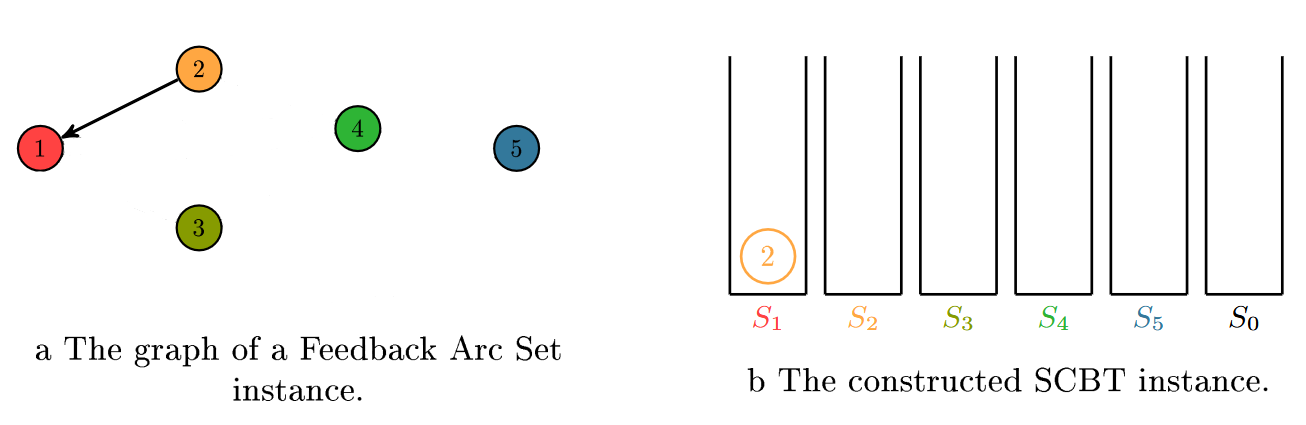
\includegraphics[width=\textwidth]{construct09}
		\caption{Konstruktion}
    \end{figure}
\end{frame}

\begin{frame}{Konstruktion}
\begin{pointlist}
\item Ein Ball der Farbe $u$ in Tube $v$ für jede Kante $(u,v)\in E$
\end{pointlist}
\begin{figure}[ht]
		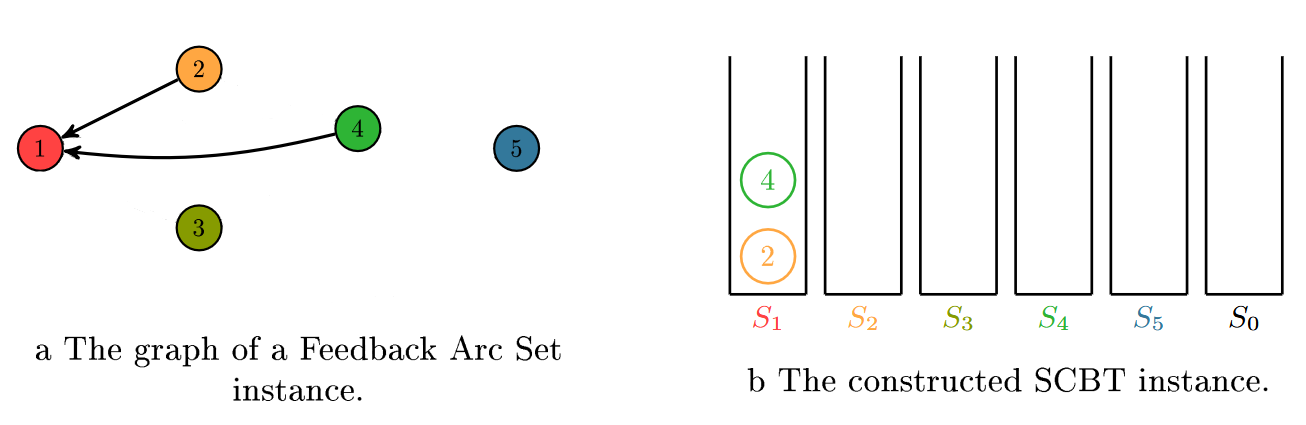
\includegraphics[width=\textwidth]{construct08}
		\caption{Konstruktion}
    \end{figure}
\end{frame}

\begin{frame}{Konstruktion}
\begin{pointlist}
\item Ein Ball der Farbe $u$ in Tube $v$ für jede Kante $(u,v)\in E$
\end{pointlist}
\begin{figure}[ht]
		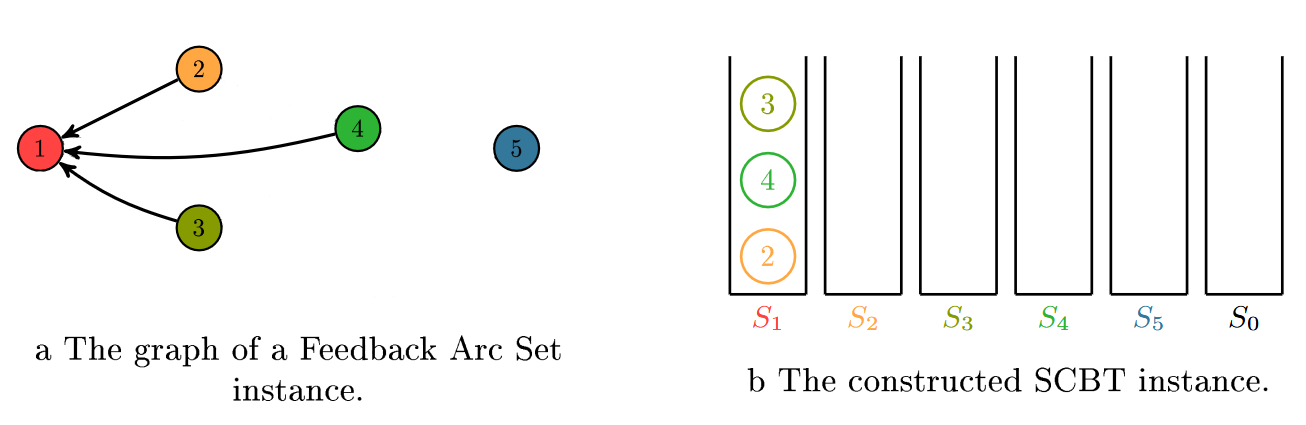
\includegraphics[width=\textwidth]{construct07}
		\caption{Konstruktion}
    \end{figure}
\end{frame}

\begin{frame}{Konstruktion}
\begin{pointlist}
\item Ein Ball der Farbe $u$ in Tube $v$ für jede Kante $(u,v)\in E$
\end{pointlist}
\begin{figure}[ht]
		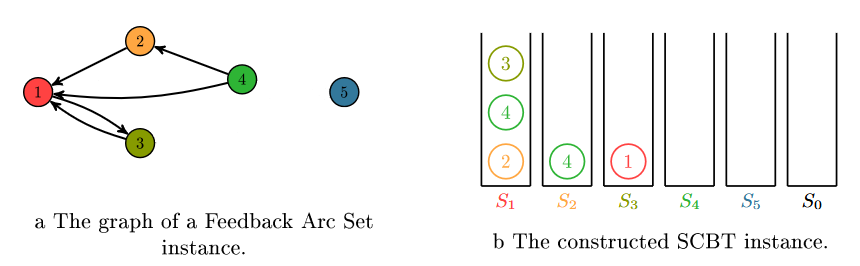
\includegraphics[width=\textwidth]{construct06}
		\caption{Konstruktion}
    \end{figure}
\end{frame}

\begin{frame}{Konstruktion}
\begin{pointlist}
\item Ein Ball der Farbe $u$ in Tube $v$ für jede Kante $(u,v)\in E$
\end{pointlist}
\begin{figure}[ht]
		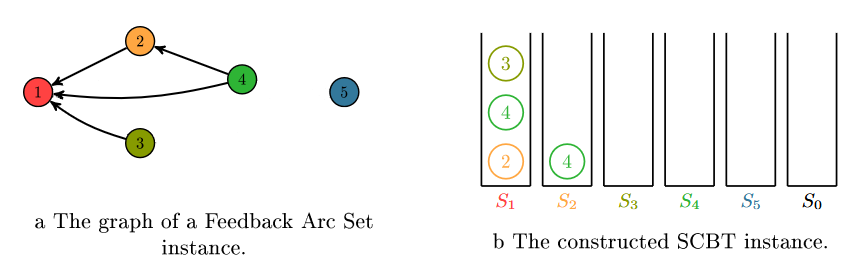
\includegraphics[width=\textwidth]{construct05}
		\caption{Konstruktion}
    \end{figure}
\end{frame}

\begin{frame}{Konstruktion}
\begin{pointlist}
\item Ein Ball der Farbe $u$ in Tube $v$ für jede Kante $(u,v)\in E$
\end{pointlist}
\begin{figure}[ht]
		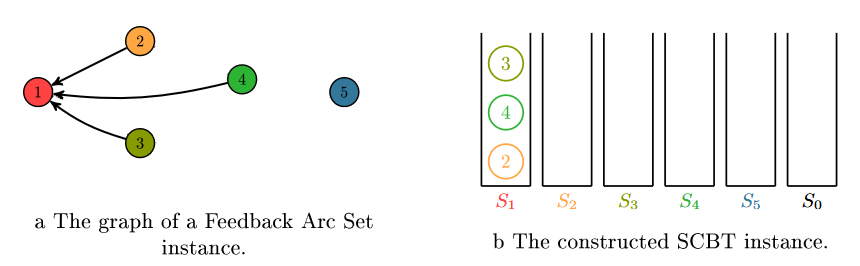
\includegraphics[width=\textwidth]{construct04}
		\caption{Konstruktion}
    \end{figure}
\end{frame}

\begin{frame}{Konstruktion}
\begin{pointlist}
\item Ein Ball der Farbe $u$ in Tube $v$ für jede Kante $(u,v)\in E$
\end{pointlist}
\begin{figure}[ht]
		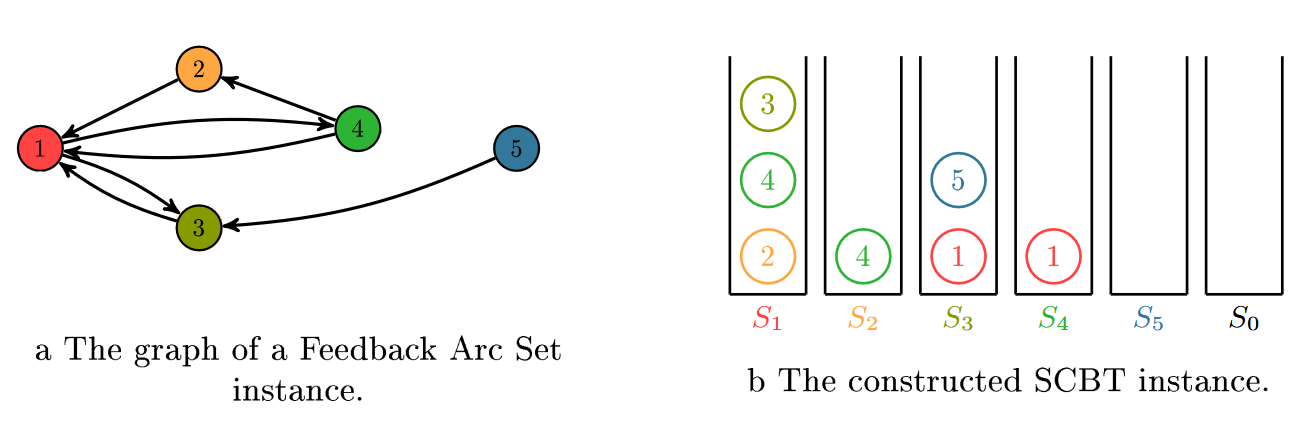
\includegraphics[width=\textwidth]{construct03}
		\caption{Konstruktion}
    \end{figure}
\end{frame}

\begin{frame}{Konstruktion}
\begin{pointlist}
\item Ein Ball der Farbe $u$ in Tube $v$ für jede Kante $(u,v)\in E$
\end{pointlist}
\begin{figure}[ht]
		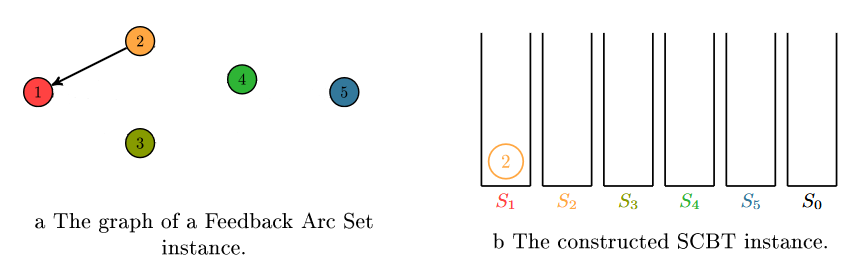
\includegraphics[width=\textwidth]{construct02}
		\caption{Konstruktion}
    \end{figure}
\end{frame}

\begin{frame}{Konstruktion}
\begin{pointlist}
\item Ein Ball der Farbe $u$ in Tube $v$ für jede Kante $(u,v)\in E$
\end{pointlist}
\begin{figure}[ht]
		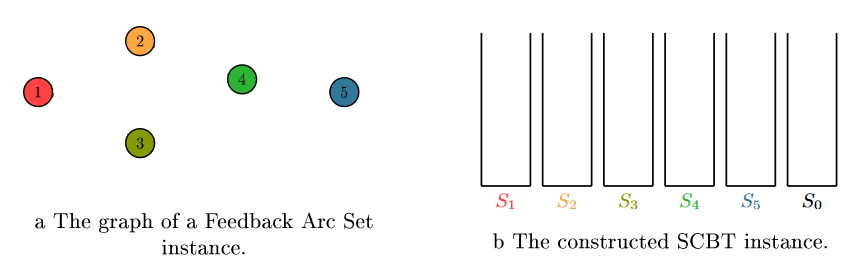
\includegraphics[width=\textwidth]{construct01}
		\caption{Konstruktion}
    \end{figure}
\end{frame}

\begin{frame}{Konstruktion}
\begin{pointlist}
\item konstruierte Instanz $((\infty, \dots, \infty), (S_u)_{u=1}^n, |E|+k)$
\end{pointlist}
\begin{figure}[ht]
		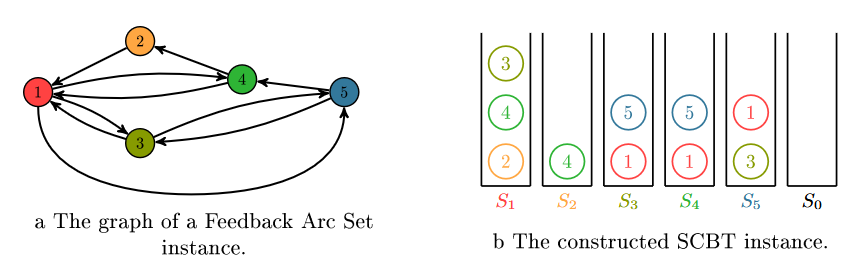
\includegraphics[width=\textwidth]{construct}
		\caption{Konstruktion}
    \end{figure}
\end{frame}

\section*{Lemma 2}
\begin{frame}{Lemma 2}
\begin{pointlist}
\item Instanz $(G,k)$ von FAS hat genau dann eine Lösung, wenn die konstruierte Instanz $((\infty, \dots, \infty), (S_u)_{u=1}^n, |E|+k)$ von SCBT eine Lösung hat
\begin{arrowlist}
\item SCBT ist auch NP-vollständig
\end{arrowlist}
\end{pointlist}
\end{frame}

\begin{frame}{Beweis (\glqq $\Rightarrow$\grqq)}
\begin{pointlist}
\item geg.: $(G,k)$ mit $G=(V,E)$
\end{pointlist}

	\begin{figure}[ht]
		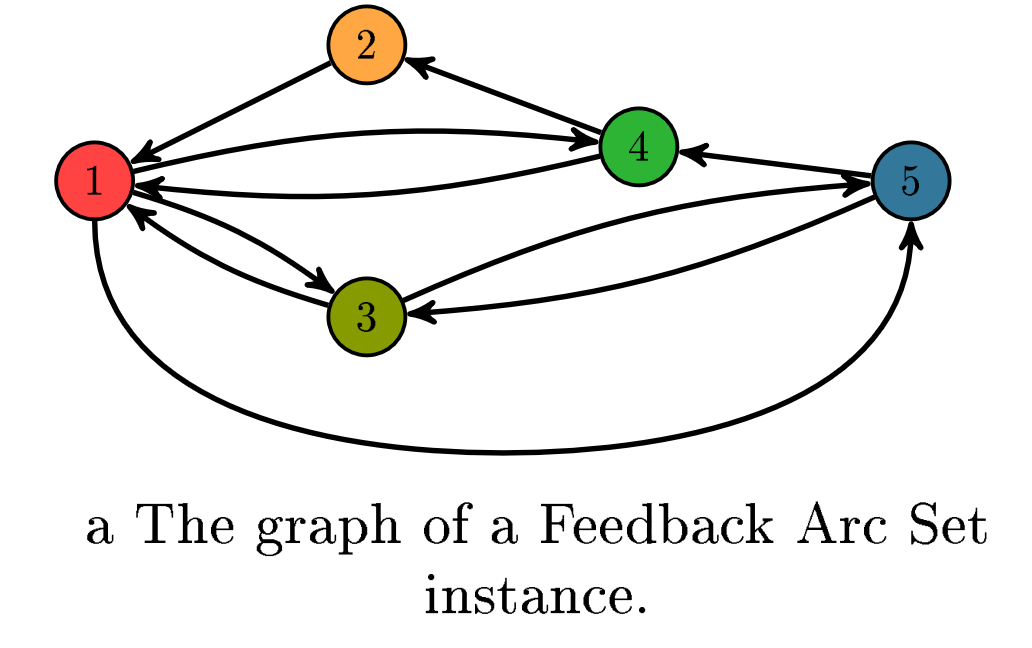
\includegraphics[width=.75\textwidth]{graph}
		\caption{Konstruktion}
    \end{figure}
\end{frame}

\begin{frame}{Beweis (\glqq $\Rightarrow$\grqq)}
\begin{pointlist}
\item Sei $E'\subseteq E$ mit $|E'| \leq k$ eine Lösung für FAS
\end{pointlist}
\begin{figure}[ht]
		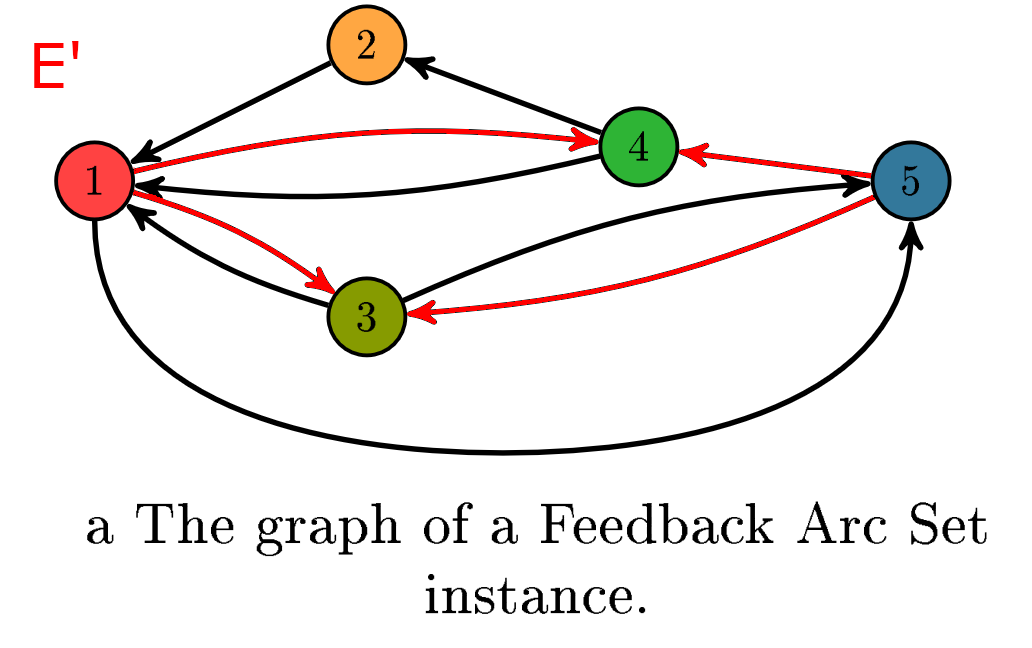
\includegraphics[width=.75\textwidth]{graphe}
		\caption{Konstruktion}
    \end{figure}
\end{frame}

\begin{frame}{Beweis (\glqq $\Rightarrow$\grqq)}
\begin{pointlist}
\item Sei $\pi:\{1,\dots,n\}\rightarrow \{1,\dots,n\}$ eine topologische Sortierung von $G'=(V, E\backslash E')$, sodass $\forall (u,v)\in E\backslash E': \pi(u)\leq \pi(v)$ 
\end{pointlist}
\begin{figure}
    \centering
    \subfloat[\centering]{{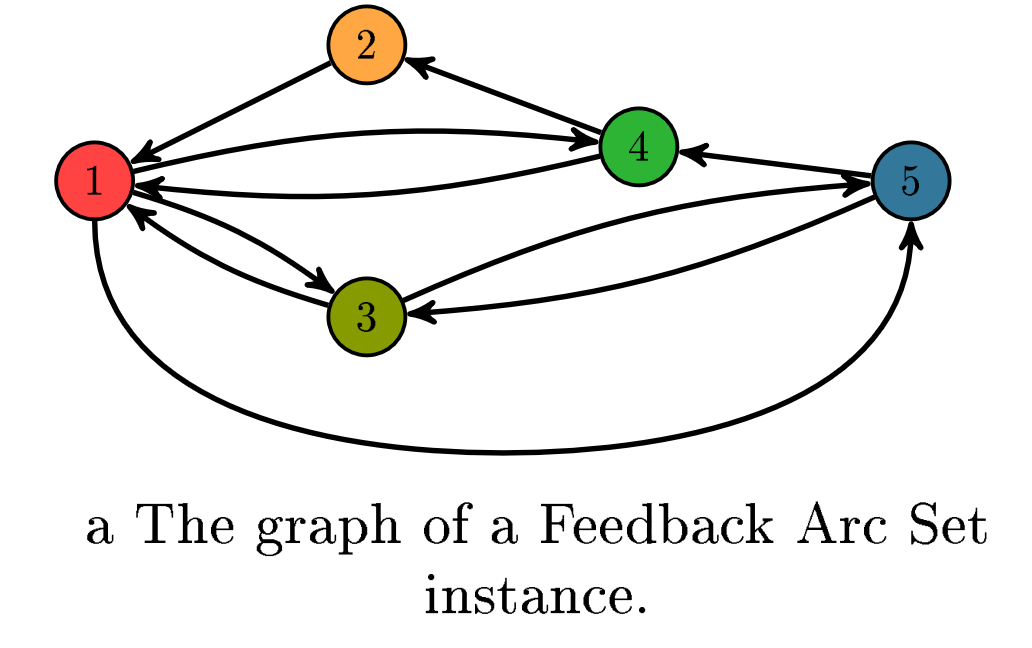
\includegraphics[width=0.48\textwidth]{graph} }}
    \subfloat[\centering]{{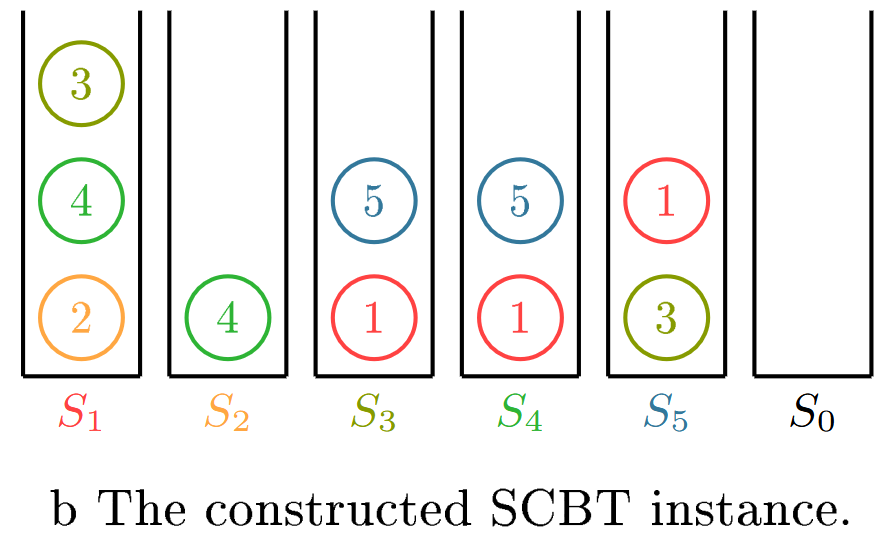
\includegraphics[width=0.48\textwidth]{constgraph} }}
\end{figure}
\end{frame}

\begin{frame}{Beweis (\glqq $\Rightarrow$\grqq)}
\begin{pointlist}
\item $\pi(4)=1$, $\pi(2)=2$, $\pi(3)=3$, $\pi(1)=4$, $\pi(5)=5$
\end{pointlist}
\begin{figure}
    \centering
    \subfloat[\centering]{{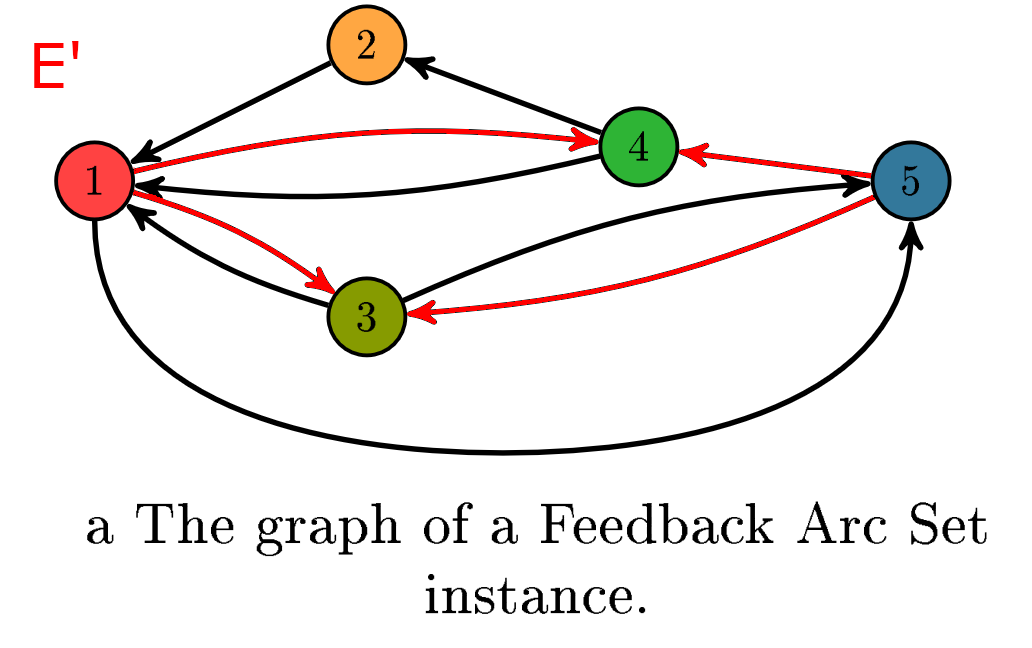
\includegraphics[width=0.48\textwidth]{graphe} }}
    \subfloat[\centering]{{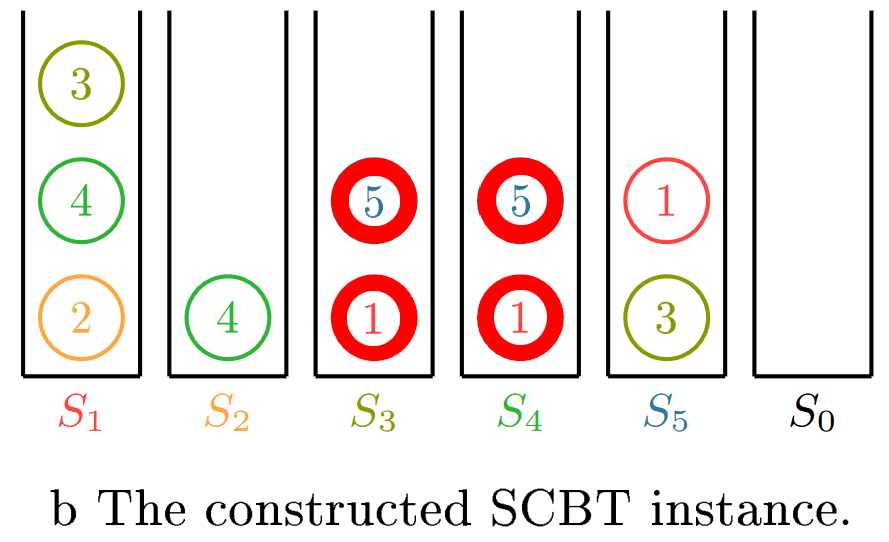
\includegraphics[width=0.48\textwidth]{constgraph2} }}
\end{figure}
\end{frame}

\begin{frame}{Beweis (\glqq $\Rightarrow$\grqq)}
\begin{pointlist}
\item Für $i=1,\dots,n$:
\begin{arrowlist}
\item Bälle in $S_{\pi(i)}$, die einer Kante aus $E'$ entsprechen, gehen in die Reserve-Tube 
\item Bälle in $S_{\pi(i)}$, die einer Kante $(\pi(i),u)\in E\backslash E'$ entsprechen, gehen in Tube $S_u$
\end{arrowlist}
\end{pointlist}
\begin{figure}
    \centering
    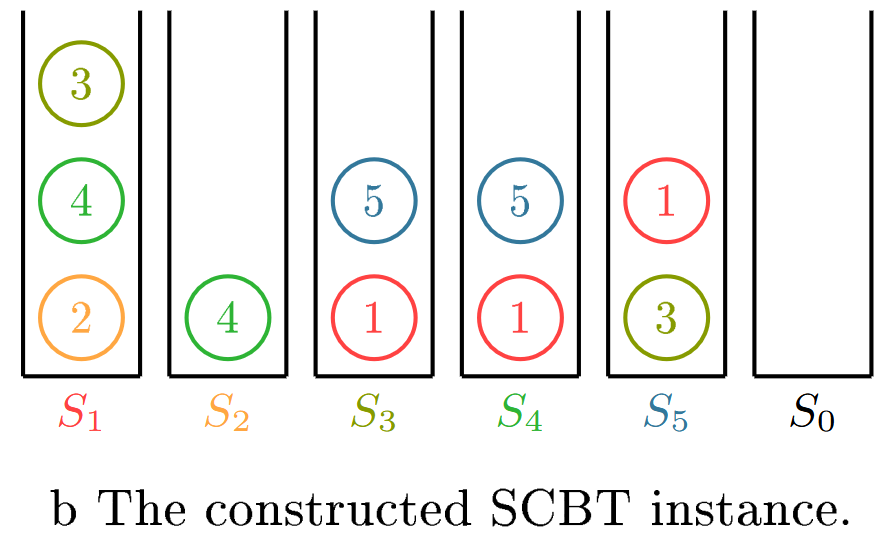
\includegraphics[width=0.65\textwidth]{constgraph}
\end{figure}
\end{frame}

\begin{frame}{Beweis (\glqq $\Rightarrow$\grqq)}
\begin{pointlist}
\item Für $i=1,\dots,n$:
\begin{arrowlist}
\item Bälle in $S_{\pi(i)}$, die einer Kante aus $E'$ entsprechen, gehen in die Reserve-Tube 
\item Bälle in $S_{\pi(i)}$, die einer Kante $(\pi(i),u)\in E\backslash E'$ entsprechen, gehen in Tube $S_u$
\end{arrowlist}
\end{pointlist}
\begin{figure}
    \centering
    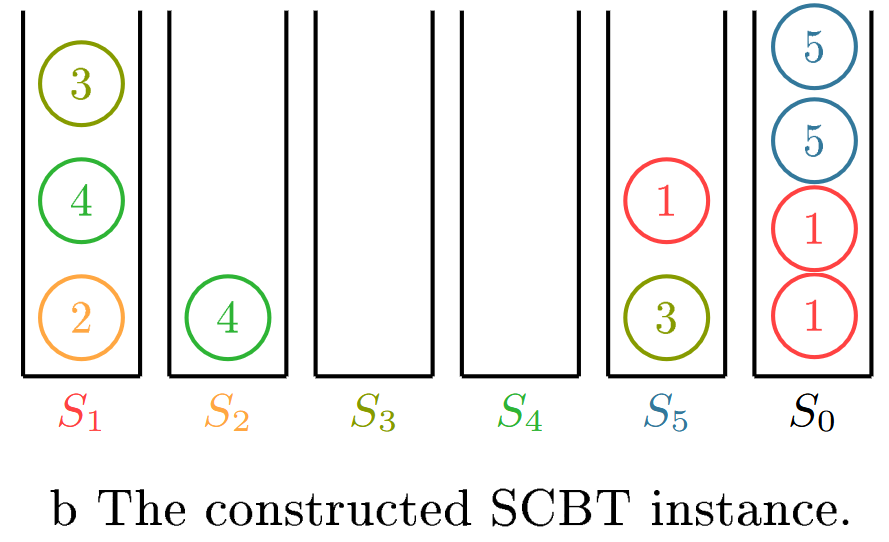
\includegraphics[width=0.65\textwidth]{proofr1}
\end{figure}
\end{frame}


\begin{frame}{Beweis (\glqq $\Rightarrow$\grqq)}
\begin{pointlist}
\item Für $i=1,\dots,n$:
\begin{arrowlist}
\item Bälle in $S_{\pi(i)}$, die einer Kante aus $E'$ entsprechen, gehen in die Reserve-Tube 
\item Bälle in $S_{\pi(i)}$, die einer Kante $(\pi(i),u)\in E\backslash E'$ entsprechen, gehen in Tube $S_u$
\end{arrowlist}
\end{pointlist}
\begin{figure}
    \centering
    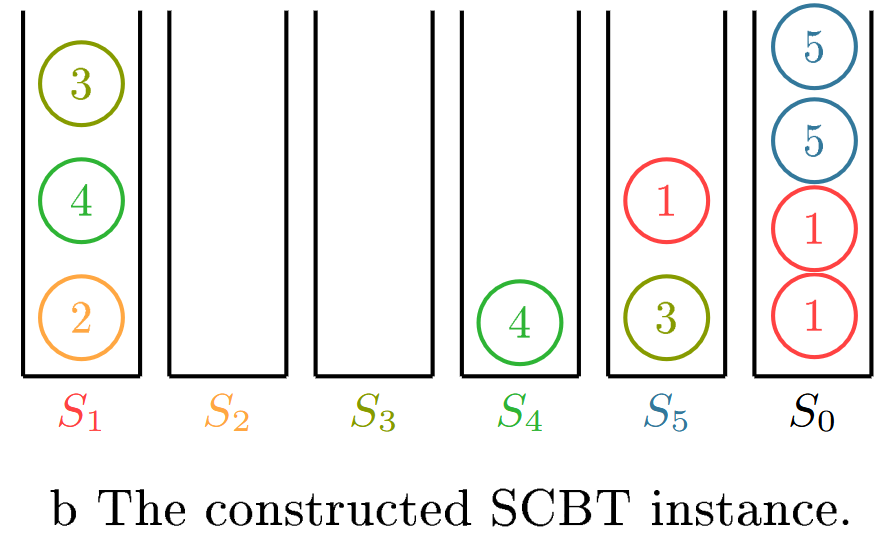
\includegraphics[width=0.65\textwidth]{proofr2}
\end{figure}
\end{frame}

\begin{frame}{Beweis (\glqq $\Rightarrow$\grqq)}
\begin{pointlist}
\item Für $i=1,\dots,n$:
\begin{arrowlist}
\item Bälle in $S_{\pi(i)}$, die einer Kante aus $E'$ entsprechen, gehen in die Reserve-Tube 
\item Bälle in $S_{\pi(i)}$, die einer Kante $(\pi(i),u)\in E\backslash E'$ entsprechen, gehen in Tube $S_u$
\end{arrowlist}
\end{pointlist}
\begin{figure}
    \centering
    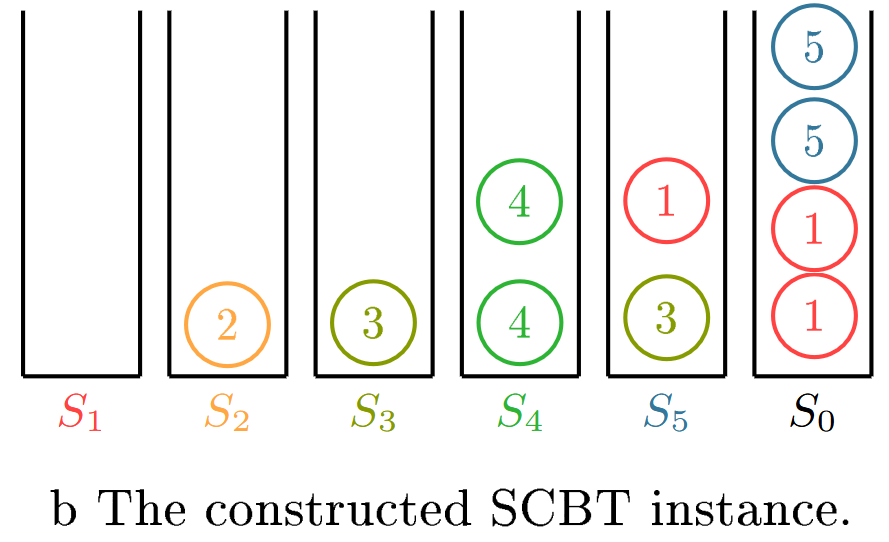
\includegraphics[width=0.65\textwidth]{proofr3}
\end{figure}
\end{frame}

\begin{frame}{Beweis (\glqq $\Rightarrow$\grqq)}
\begin{pointlist}
\item Für $i=1,\dots,n$:
\begin{arrowlist}
\item Bälle in $S_{\pi(i)}$, die einer Kante aus $E'$ entsprechen, gehen in die Reserve-Tube 
\item Bälle in $S_{\pi(i)}$, die einer Kante $(\pi(i),u)\in E\backslash E'$ entsprechen, gehen in Tube $S_u$
\end{arrowlist}
\end{pointlist}
\begin{figure}
    \centering
    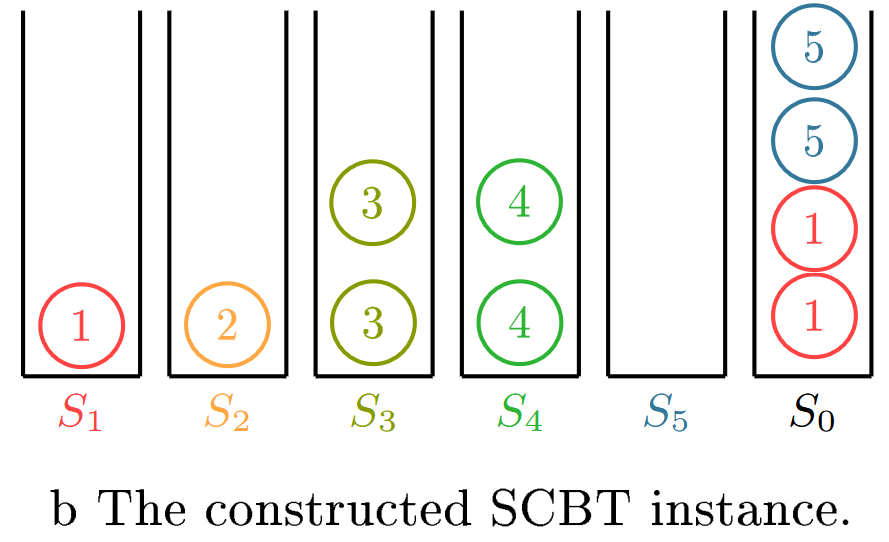
\includegraphics[width=0.65\textwidth]{proofr4}
\end{figure}
\end{frame}

\begin{frame}{Beweis (\glqq $\Rightarrow$\grqq)}
\begin{pointlist}
\item Durch die topologische Sortierung ist die Tube $S_u$ die finale für den jeweiligen Ball, daher $k_1 = |E\backslash E'|$ viele Züge
\item Die Bälle in der Reserve-Tube werden schließlich auf ihre Farben aufgeteilt, daher $k_2 = 2\cdot |E'|$ viele Züge
\item $k_1 + k_2 =  |E\backslash E'| + 2\cdot |E'| = |E| + |E'| \leq |E| + k$
\item Konstruierte Instanz $((\infty, \dots, \infty), (S_u)_{u=1}^n, |E|+k)$ hat eine Lösung
\end{pointlist}
\begin{figure}
    \centering
    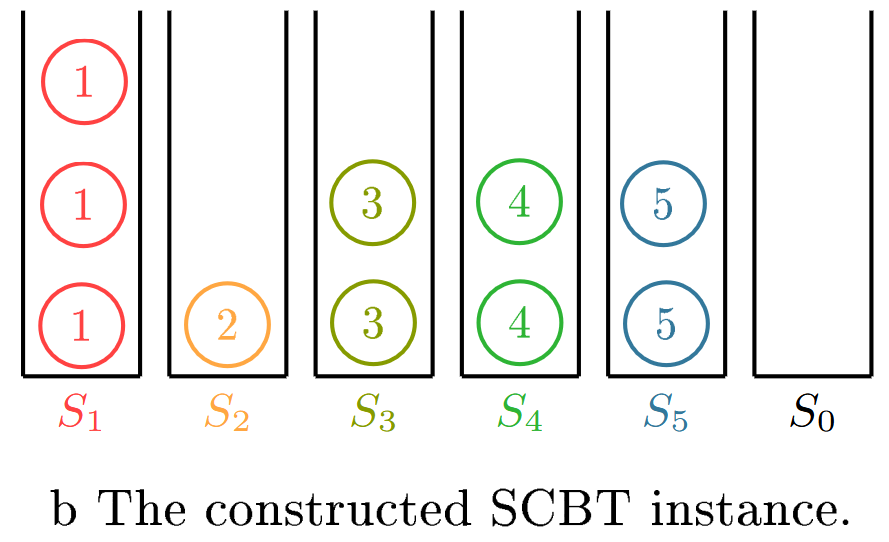
\includegraphics[width=0.65\textwidth]{proofr5}
\end{figure}
\end{frame}

\begin{frame}{Beweis (\glqq $\Leftarrow$\grqq)}
\begin{pointlist}
\item geg.: Konstruierte Instanz kann in $|E|+k$ Zügen gelöst werden
\item Lemma 1. besagt, dass jeder Ball entweder einmal final bewegt wird oder zuerst in die Reserve-Tube geht
\item Sei $E'$ die Menge mit Bällen, die 2-mal bewegt werden
\item Jeder Ball muss mindestens 1-mal bewegt werden, somit $|E|$
\item Jeder zusätzlicher Zug fällt unter $k$, daher $|E'|\leq k$
\end{pointlist}
\end{frame}

\begin{frame}{Beweis (\glqq $\Leftarrow$\grqq)}
\begin{pointlist}
\item Annahme: $G'=(V,E\backslash E')$ hat einen Zyklus
\item Ball für Kante $(u,v)\in E\backslash E'$ kann erst final bewegt werden, wenn alle Bälle in Zielröhre $S_u$ entfernt wurden
\item Der Ball kann nur bewegt werden, wenn ein anderer im Zyklus bewegt werden kann $\lightning$ 
\begin{arrowlist}
\item $G'=(V,E\backslash E')$ ist azyklisch 
\end{arrowlist}
\end{pointlist}
\begin{figure}
    \centering
    \subfloat[\centering]{{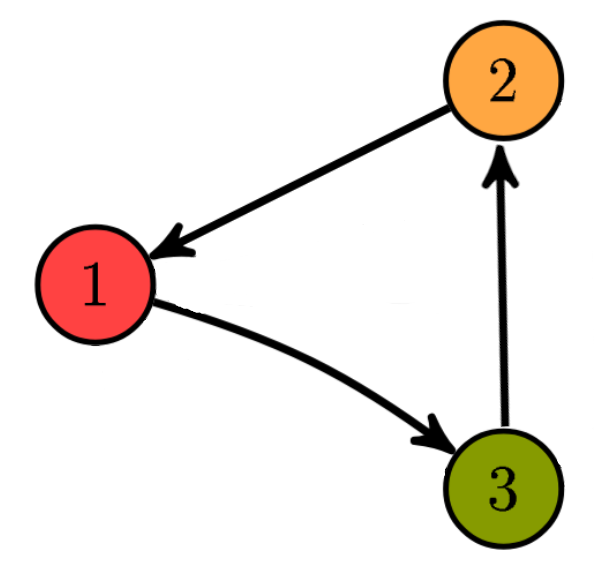
\includegraphics[width=0.3\textwidth]{zykg} }}
    \qquad
    \subfloat[\centering]{{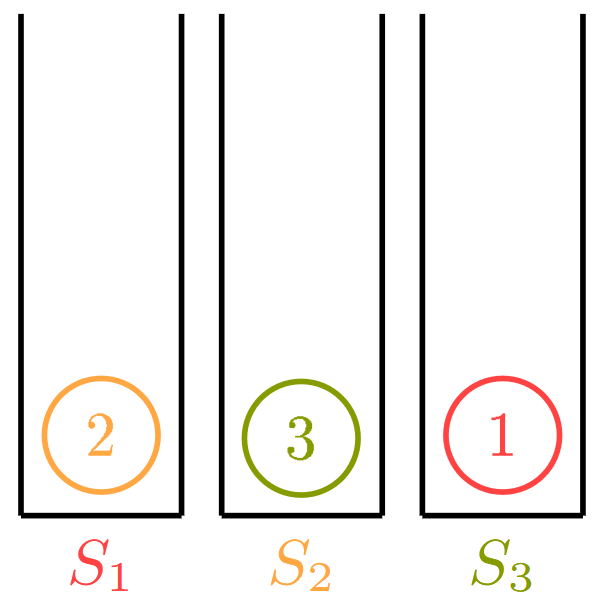
\includegraphics[width=0.3\textwidth]{zyk} }}
\end{figure}
\end{frame}

\section*{RSCBT}
\begin{frame}{Restricted SCBT (RSCBT)}
\begin{pointlist}
\item Das RSCBT Problem ist auch NP-vollständig
\end{pointlist}
\end{frame}

\section*{Idee}
\begin{frame}{Idee}
\begin{pointlist}
\item Um einen schnelleren Algorithmus zu bekommen, wollen wir eine untere Schranke bestimmen
\item Damit müssen wir in der Breiten Suche die Konfigurationen nicht nummerieren, da wir wissen wie viele Züge minimal nötig sind
\item Über ein Directed Feedback Vertex Set (DFVS) Solver berechnen wir eine untere Schranke
\end{pointlist}
\end{frame}

\section*{DFVS}
\begin{frame}{Directed Feedback Vertex Set (DFVS)}
\begin{pointlist}
\item geg.: gerichteter Graph G=(V,E) und Integer $k$
\item ges.: $\exists V' \subseteq V$ mit $|V'|\leq k$, sodass $G'[V\backslash V']$ azyklisch ist
\begin{arrowlist}
\item NP-vollständig
\end{arrowlist}
\end{pointlist}
\end{frame}

\section*{Lower Bounds}
\begin{frame}{Lower Bounds}
\begin{pointlist}
\item Untere Schranke kann berechnet werden, da das Hinzufügen von Einschränkungen die Anzahl an Zügen nicht verringern kann
\item FAS-Instanz wird auf eine DFVS-Instanz reduziert
\item Diese Instanz wird mit für kleinere $k$ mit einem $DFVS$-Solver gelöst
\item Untere Schranke wird experimentell berechnet
\end{pointlist}
\end{frame}


\section*{Algo}
\begin{frame}{Algorithmus}
\begin{figure}
    \centering
    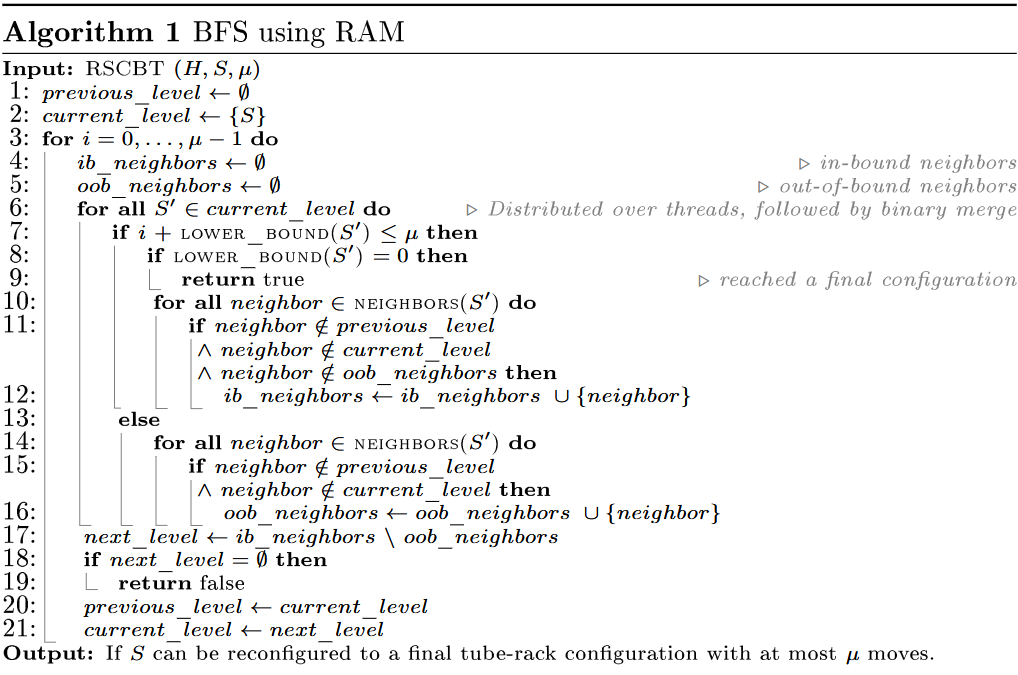
\includegraphics[width=\textwidth]{algo}
\end{figure}
\end{frame}

\section*{Experiment}
\begin{frame}{Experimente}
\begin{figure}
    \centering
    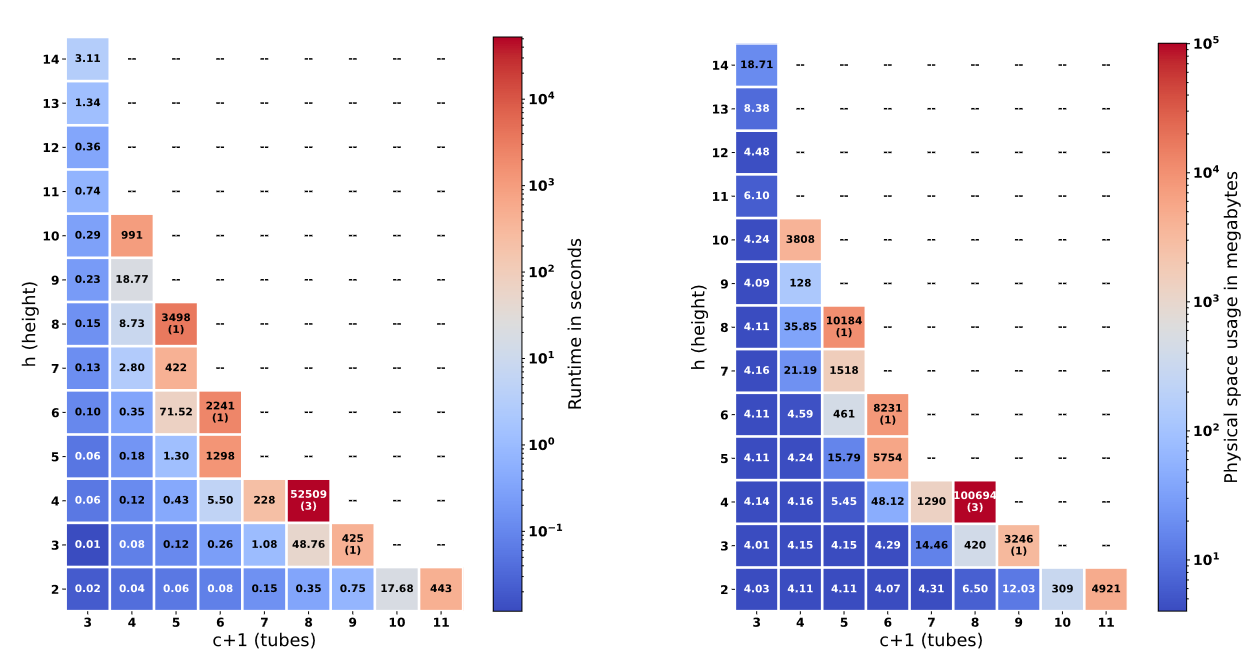
\includegraphics[width=\textwidth]{topexp}
\end{figure}
\end{frame}


\begin{frame}{Experimente}
\begin{figure}
    \centering
    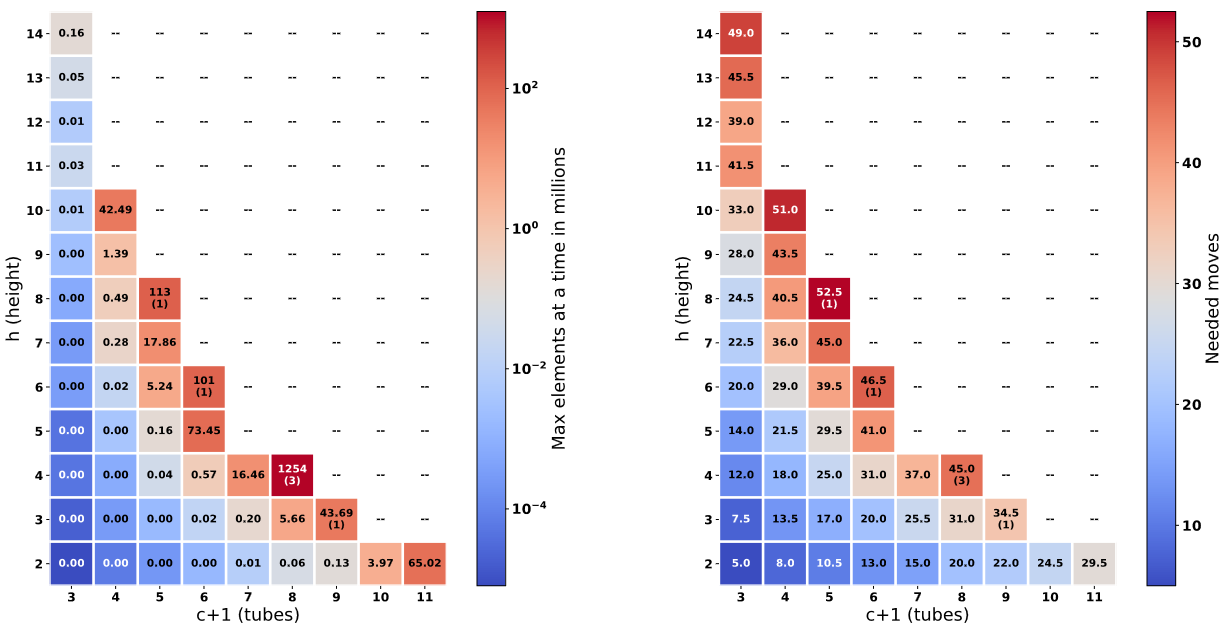
\includegraphics[width=\textwidth]{botexp}
\end{figure}
\end{frame}

\begin{frame}{}
  \centering \Huge
  \emph{Fin}
\end{frame}


	
    	
    	
    	
\end{document}
